Proper evaluation methods guide researchers in choosing the model that best fits their needs; thus, this chapter is dedicated to the most common evaluation metrics adopted by academics in the field of EF. Error metrics and measures vary depending on wethter we are concerned with point or probabilistic forecasts. Additionally, note that the latter can take different forms which therefore requires different measures.
\section{MAE}\label{mae}
Consider the time series with actual values given by $\mathrm{L}=(L_{n+1}, L_{n+2},\dots, L_{n+h})$
and its h step ahead point forecast $\mathrm{\hat{L}}=(\hat{L}_{n+1}, \hat{L}_{n+2},\dots, \hat{L}_{n+h})$ the mean absolute error is defined as
\begin{definition}
    $\mathrm{MAE}(\mathrm{L},\mathrm{\hat{L}})=\frac{1}{h}\|\mathrm{L}-\mathrm{\hat{L}}\|_{1}=\frac{1}{h}\sum\limits_{k=1}^{h}|L_{n+k}-\hat{L}_{n+k}|$
\end{definition}

\section{RMSE}\label{rmse}
\begin{definition}
    $\mathrm{RMSE(\mathrm{L}, \mathrm{\hat{L}})}=\frac{1}{\sqrt{h}}\|\mathrm{L}-\mathrm{\hat{L}}\|_{2}=\sqrt{\frac{\sum\limits_{k=1}^{h}(L_{n+k}- \hat{L}_{n+k})^2}{h}}$
\end{definition}

MAE and RMSE posses the useful property of being expressed in the same units of the data thus enabling meaningful comparisons.
However, a drawback of such measures is that we cannot use them to compare accuracy between time series wich have different magnitudes. For instance, a day ahead error of 1kWh is negligible when considering a daily demand of 100kWn while the same error is considerably big when daily demand is 2kWh. This consideration leads to relative accuracy scores, between those the MAPE is by far the most popular.


\section{MAPE}\label{mape}. 
\begin{definition}
    $\mathrm{MAPE}(\mathrm{L},\mathrm{\hat{L}})=\frac{100}{h}\sum\limits_{k=1}^{h}\frac{|L_{n+k}-\hat{L}_{n+k}|}{|L_{n+k}|}$
\end{definition}

\section{RMSPE}\label{rmspe}
\begin{definition}
    $\mathrm{RMSPE}(\mathrm{L},\mathrm{\hat{L}})=100\cdot\sqrt{\frac{1}{h}\sum\limits_{k=1}^{h} \left(\frac{|L_{n+k}-\hat{L}_{n+k}|}{|L_{n+k}|}\right)^2}$
\end{definition}
Note, MAPE and RMSPE may not be appropriate for series which have zero or very small values, for example, electricity demand at the household level; the result is a large score regardless of the absolute errors.
Scaled errors constitute a robust family of scores.
\section{MASE}\label{mase}
\begin{definition}
    $\mathrm{MASE}(\mathrm{L},\mathrm{\hat{L}})=\frac{1}{h}\sum\limits_{k=1}^N\frac{|L_{n+k}-\hat{L}_{n+k}|}{\frac{1}{h-1}\sum\limits_{k=2}^{h}|L_{k}-L_{k-1}|}$
\end{definition}
In the denominator we have the error of the naïve/persistence model. 
In this model, the current demand makes up the prediction for the next time step; that is $\mathrm{\hat{L}^{\mathrm{naive}}}_{n+1}=\mathrm{L}_{n}$.
\section{RMSSE}\label{rmsse}
\begin{definition}
    $\mathrm{RMSSE}(\mathrm{L},\mathrm{\hat{L}})=\sqrt{\frac{1}{h}\sum\limits_{k=1}^N\left(\frac{|L_{n+k}-\hat{L}_{n+k}|}{\frac{1}{h-1}\sum\limits_{k=2}^{h}|L_{k}-L_{k-1}|}\right)^2}$
\end{definition}


\section{Pinball}\label{pinball}
The pinball score or quantile score is used to measure the accuracy of a quantile forecast.
\begin{definition}
    $\mathrm{Pinball}(L_{t},\hat{L}_{t,q},q)=
\begin{cases}
(1-q)(\hat{L}_{t,q}-L_{t}) & L_t < \hat{L}_{t,q} \\
q(L_t-\hat{L}_t,q) & L_t \geq \hat{L}_{t,q}
\end{cases}$
\end{definition}
The pinball loss is an asymmetric function, it weights its score differently depending on the error sign and on the quantile considered, see \ref{fig:pinball}.
\begin{figure}
    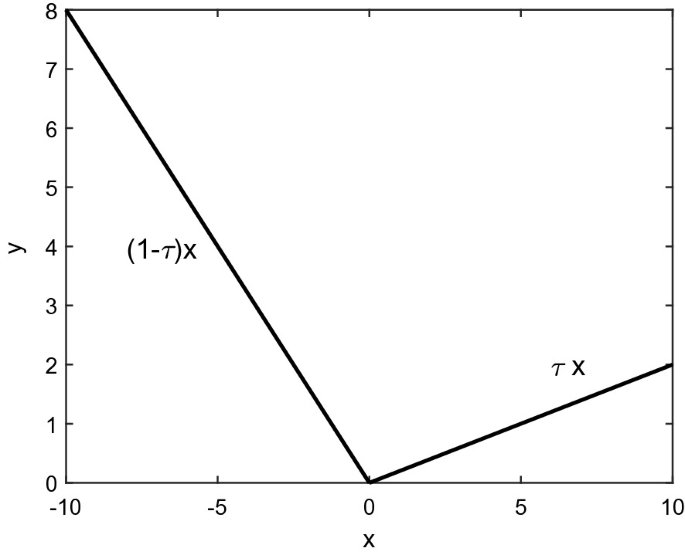
\includegraphics[width=\textwidth]{images/pinball_loos.png}
    \caption{Pinball loss with q=0.2 \cite{haben2023core}}
    \label{fig:pinball}
  \end{figure}
By averaging all the pinball losses over all quantiles and over the whole forecast horizon, we obtain the pinball loss of the probabilistic forecast.
\section{Winkler}
\begin{definition}
    $\mathrm{Winkler}_{\alpha}=\begin{cases}
        \delta & Low_{t}\leq L_{t}\leq Upp{t}\\
        \delta+2(Low_{t}-L_{t})/\alpha & L_{t}<Low_{t}\\
        \delta+2(L{t}-Upp_{t})/\alpha & L_{t} \geq Upp_{t}
    \end{cases}$
\end{definition}
Where delta is the PI width, that is $\delta=Upp_t-Low_t$. This score penalizes observations falling outside the PI and rewards narrow PI.
\section{CRPS}
The continous ranked probability score measures the differece between the estimated cumulative distribution $\hat{F}$ and the empirical Cdf.
\begin{definition}\label{def_crps}
    $\mathrm{CRPS}(L, \hat{F})=\int\limits_{-\infty}^{\infty}\left(\hat{F}(x)-\mathbb{1}(x-L) \right)^2 dx$
\end{definition}
Nevertheless, we can evaluate the integral in closed form. 
Where the indicator function is defined as 
    $\mathbb{1}(z)=
\begin{cases}
0 & z<0\\
1 & z \geq 0
\end{cases}$
\\
For a visualisation see, \ref{fig:crps}. The grey area is what contributes toward the CRPS score.
The better the estimated cdf is the smaller the total CRPS score will be.
\begin{figure}
    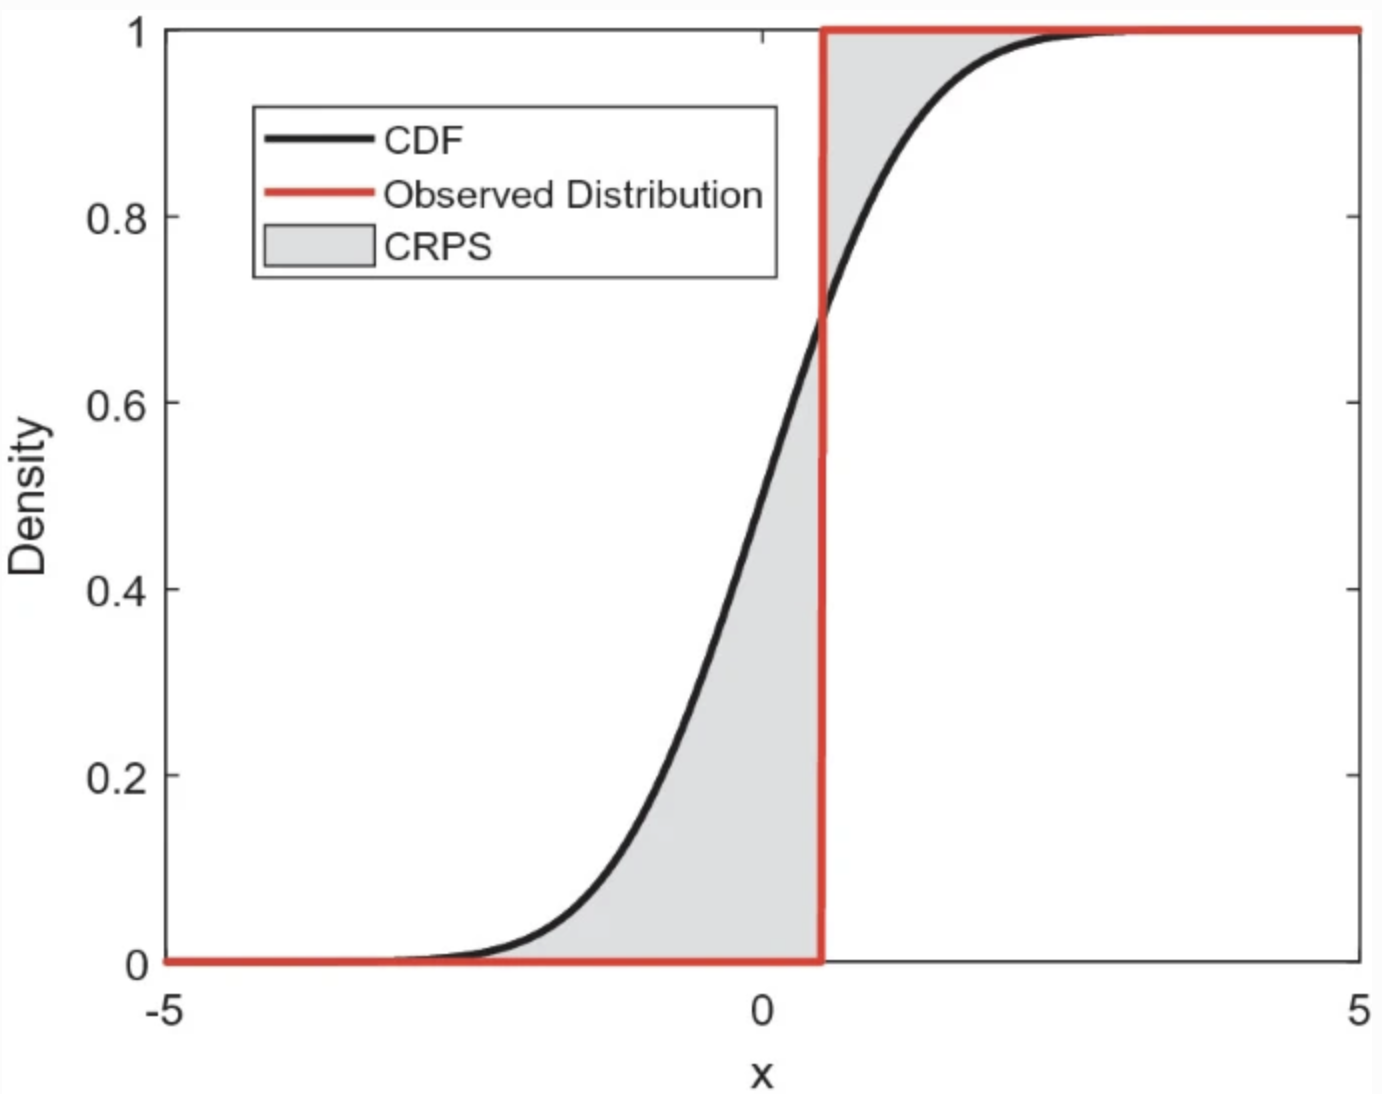
\includegraphics[width=\textwidth]{images/crps.png}
    \caption{CRPS integral \cite{haben2023core}}
    \label{fig:crps}
  \end{figure}
  \\
It is worth noting, that the CRPS integral can be rewritten in terms of expectations. This makes its evaluation easier, since we know that the sample mean converges to the expectation by the law of large numbers. This was first pointed out by \cite{proper_scores}, where authors take advantage of lemma 2.2 of \cite{new_multi_test2} or equivalently identity 17 of \cite{new_multi_tes1}.
\\
\begin{lemma}
    Let $\mathrm{X}_1$, $\mathrm{X}_2$, $\mathrm{Y}_1$, $\mathrm{Y}_2$ be independent real random variables with finite expectations. Let $\mathrm{X}_1,\mathrm{X}_2$ be identically distributed with distribution function $\mathrm{F}$ and let $\mathrm{Y}_1,\mathrm{Y}_2$ be identically distributed with distribution function $\mathrm{G}$. Then
   \begin{equation}
    \mathbb{E}(|X_1-Y_1|)-\frac{1}{2}\mathbb{E}(|X_1-X_2|)-\frac{1}{2}\mathbb{E}(|Y_1-Y_2|)=\int\limits_{-\infty}^{\infty}\left(F(x)-G(x)\right)^2dx
\end{equation}
\end{lemma}
Notice that, in our case  \ref{def_crps}, the distribution $G$ of $Y_1$ and $Y_2$ is degenerate, with all probability mass on a single point.
%  (x notation will need to be cleaned here). Since $G(t)=:$
It follows that, the third addend in the summation is zero. That is because the fact of $Y_1$ and $Y_2$ both following distribution $G$ implies that $\mathbb{E}(|Y_1-Y_2|)$ corresponds to the difference of two equal constant numbers.
\\
Additionally, since $Y_1$ is just a constant, we have $Y_1=L$.
\\
Putting everything together we have obtained an alternative way of computing the CRPS score.
\begin{equation}
    \int\limits_{-\infty}^{\infty}\left(\hat{F}(x)-\mathbb{1}(x-L) \right)^2 dx=\mathbb{E}(|X_1-L|)-\frac{1}{2}\mathbb{E}(|X_1-X_2|)
\end{equation}
\\
\section{PIT}
The probability integral transform is a method to assess visually the quality of probabilistic forecasts. PIT is obtained by applying a cdf $F$ to your data; if applying such cdf to the data results in a uniform distributed PIT then $F$ is a valid prediction. If not, $F$ is not the suited cdf for the considered data. Figure \ref{fig:pit} provides an example, applying the true cdf results in a well calibrated PIT (left). Alternatively, applying a bad cdf results in either a overdispersed (middle) or underdispersed (right) PIT.
\begin{figure}
    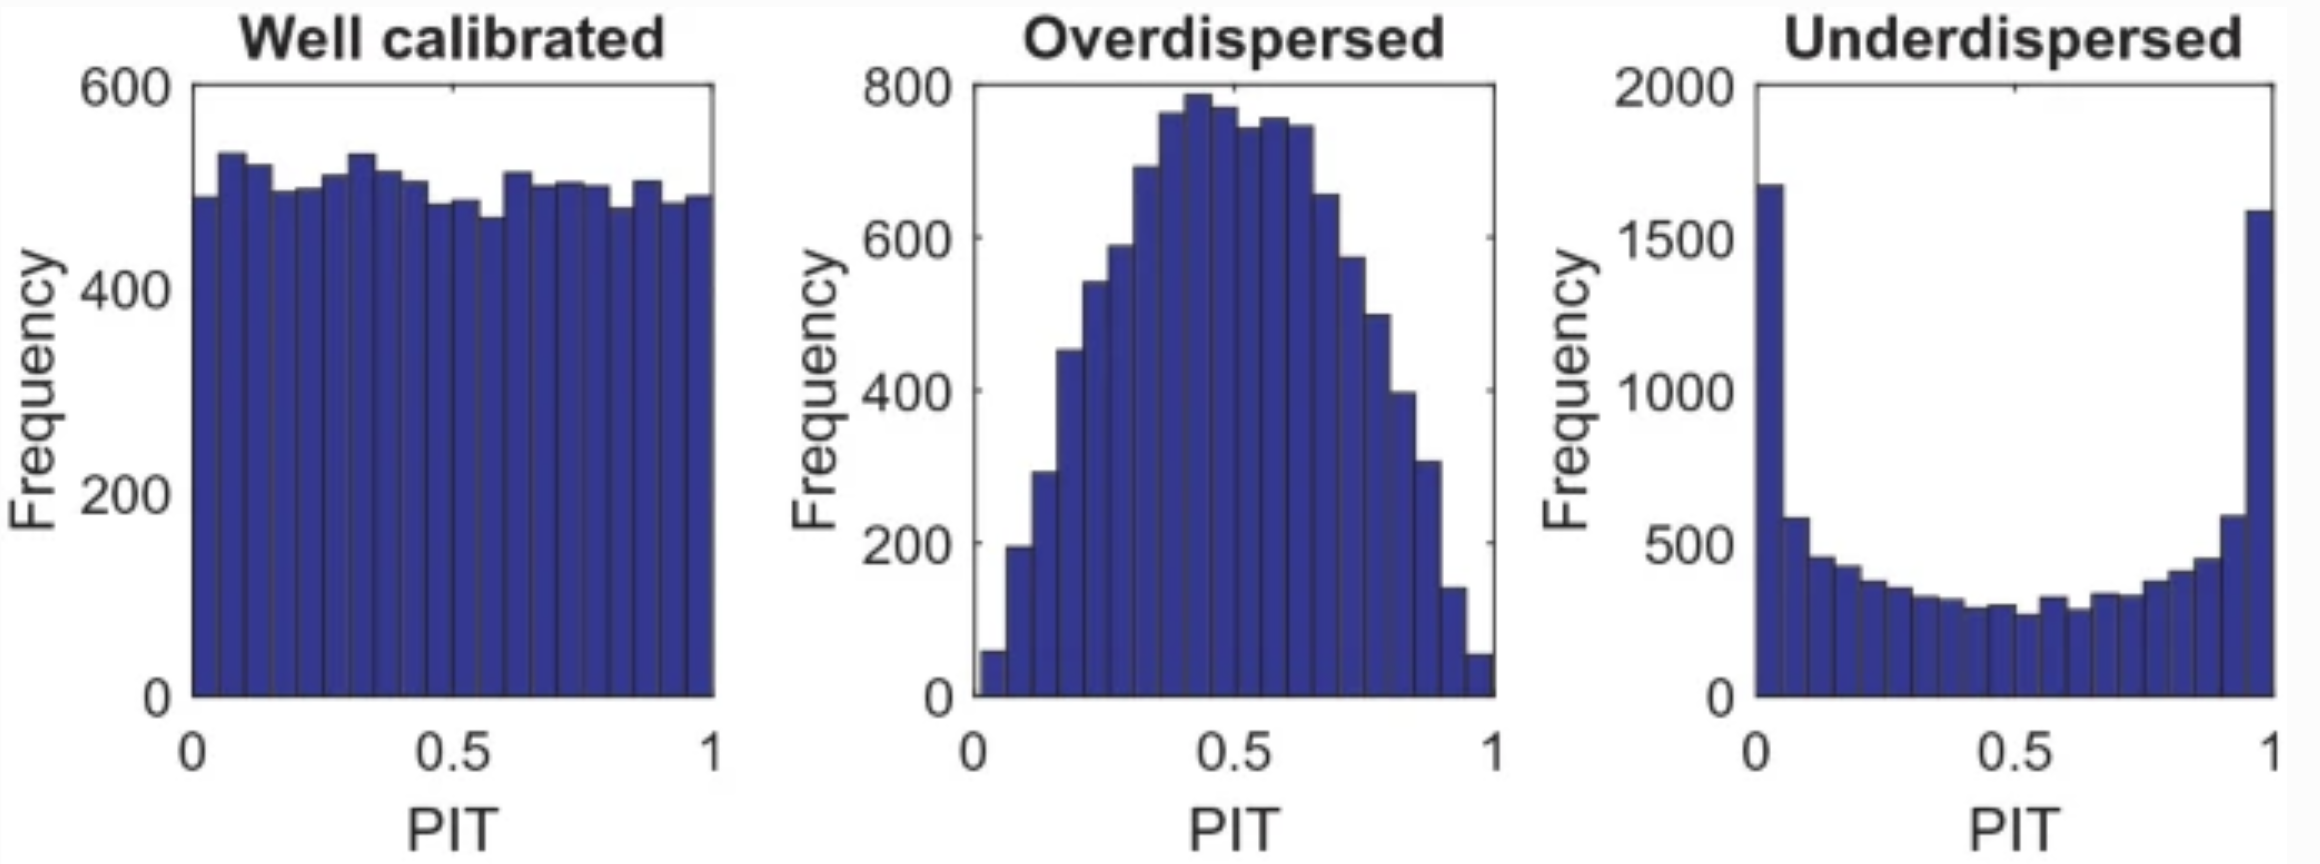
\includegraphics[width=\textwidth]{images/pit.png}
    \caption{PIT types \cite{haben2023core}}
    \label{fig:pit}
  \end{figure}
\\
%RELIABILITY PLOT
%PICP,NMPIW,CWC,unconditional coverage(arora)-->Probability density forecasting of wind speed based on quantile regression and kernel density estimation Lei Zhang

% Reliability and sharpness \section{Criteria}-->Recent advances in electricity price forecsating a review of probabilistic forecasting Weron
% Two criteria are used in literature to evaluate probabilistic forecasting: sharpness and reliability. Reliability means 